%% Copernicus Publications Manuscript Preparation Template for LaTeX Submissions
%% ---------------------------------
%% This template should be used for copernicus.cls
%% The class file and some style files are bundled in the Copernicus Latex Package, which can be downloaded from the different journal webpages.
%% For further assistance please contact Copernicus Publications at: production@copernicus.org
%% https://publications.copernicus.org/for_authors/manuscript_preparation.html


%% Please use the following documentclass and journal abbreviations for discussion papers and final revised papers.

%% 2-column papers and discussion papers
\documentclass[gmd, manuscript]{copernicus}



%% Journal abbreviations (please use the same for discussion papers and final revised papers)


% Advances in Geosciences (adgeo)
% Advances in Radio Science (ars)
% Advances in Science and Research (asr)
% Advances in Statistical Climatology, Meteorology and Oceanography (ascmo)
% Annales Geophysicae (angeo)
% Archives Animal Breeding (aab)
% ASTRA Proceedings (ap)
% Atmospheric Chemistry and Physics (acp)
% Atmospheric Measurement Techniques (amt)
% Biogeosciences (bg)
% Climate of the Past (cp)
% DEUQUA Special Publications (deuquasp)
% Drinking Water Engineering and Science (dwes)
% Earth Surface Dynamics (esurf)
% Earth System Dynamics (esd)
% Earth System Science Data (essd)
% E&G Quaternary Science Journal (egqsj)
% Fossil Record (fr)
% Geographica Helvetica (gh)
% Geoscientific Instrumentation, Methods and Data Systems (gi)
% Geoscientific Model Development (gmd)
% History of Geo- and Space Sciences (hgss)
% Hydrology and Earth System Sciences (hess)
% Journal of Micropalaeontology (jm)
% Journal of Sensors and Sensor Systems (jsss)
% Mechanical Sciences (ms)
% Natural Hazards and Earth System Sciences (nhess)
% Nonlinear Processes in Geophysics (npg)
% Ocean Science (os)
% Primate Biology (pb)
% Proceedings of the International Association of Hydrological Sciences (piahs)
% Scientific Drilling (sd)
% SOIL (soil)
% Solid Earth (se)
% The Cryosphere (tc)
% Web Ecology (we)
% Wind Energy Science (wes)


%% \usepackage commands included in the copernicus.cls:
%\usepackage[german, english]{babel}
%\usepackage{tabularx}
%\usepackage{cancel}
%\usepackage{multirow}
%\usepackage{supertabular}
%\usepackage{algorithmic}
%\usepackage{algorithm}
%\usepackage{amsthm}
%\usepackage{float}
%\usepackage{subfig}
%\usepackage{rotating}


\begin{document}

\title{Update of the ozone dry deposition in the OsloCTM3 v1.0}


% \Author[affil]{given_name}{surname}

\Author[1]{Stefanie}{Falk}
\Author[2,a]{Amund}{S{\o}vde Haslerud}
%\Author[]{}{}

\affil[1]{Department of Geosciences, University of Oslo, Oslo, Norway}
\affil[2]{CICERO Center for International Climate Research, Oslo, Norway}
\affil[a]{Kjeller Vindteknikk, Kjeller, Norway}

%% The [] brackets identify the author with the corresponding affiliation. 1, 2, 3, etc. should be inserted.



\runningtitle{Update of ozone dry deposition in OsloCTM3}

\runningauthor{Falk}

\correspondence{Stefanie Falk (stefanie.falk@geo.uio.no)}



\received{}
\pubdiscuss{} %% only important for two-stage journals
\revised{}
\accepted{}
\published{}

%% These dates will be inserted by Copernicus Publications during the typesetting process.


\firstpage{1}

\maketitle



\begin{abstract}
  Since the industrial revolution, tropospheric background ozone concentrations have been increasing in the northern hemisphere. In recent years, the number of episodes of peak concentrations has been decreasing in North America and Europe due to the implementation of air quality regulations. At the same time, fast developing countries, like e.g., China or India, saw a significant increase in ozone related air pollution. High concentrations of ozone in ambient air are hazardous not only to humans but to the ecosystem in general. The impact of ozone damage on vegetation and agricultural plants in combination with advancing climate change may affect food security in the future. While the future scenarios in themselves are uncertain, there are limiting factors constraining the accuracy of surface ozone modeling also at present: The distribution and amount of precursor/decomposing species, the stratosphere-troposphere exchange as well as scavenging processes. Removal of any gas through gravitational settling or by uptake by plants and soil is referred to as dry deposition. The process of dry deposition is important for predicting surface ozone concentrations and understanding the observed amount and increase of tropospheric background ozone. The conceptual dry deposition velocities are calculated following a resistance-analogous approach wherein aerodynamic, quasi laminar, and canopy resistances are key components, but these are hard to measure explicitly. In this paper, we present the update from an empirical dry deposition parameterization to a more process based implementation in the OsloCTM3. Our focus lies mainly on a stomatal conductance-based description of the canopy resistance. We evaluate the resulting modeled ozone dry deposition with respect to observations and multi-model studies. We will also estimate the impact of a set of parameters on the modeled ozone concentrations, both at the surface and in the free troposphere. We show that ozone dry deposition decreases with respect to the previous version, leading to an increase in surface ozone of up to ??\,\unit{\%}. {\bf TODO: Finish the results section as soon as there are results.}
\end{abstract}


%\copyrightstatement{TEXT}
\introduction  %% \introduction[modified heading if necessary]
Ozone is an important trace gas for all lifeforms on Earth. Depending on the place of its occurrence it has either a positive or negative connotation. In the stratosphere, ozone absorbs most of the ultraviolet (UV)-light from the sun within the range of 100--315\,\unit{nm}, thus shielding the Earth's surface from the most harmful UV-radiation. In addition, ozone is a potent greenhouse gas in both, stratosphere and troposphere. With a radiative forcing of $0.40 \pm 0.20\,\unit{Wm^{-2}}$, it is placed third, only surpassed by \chem{CO_2} and \chem{CH_4} \citep[Chapter 8]{IPCC2013}.\\
In the troposphere and in particular in ambient air, ozone is considered as a highly toxic pollutant. Continuously high concentrations of ambient air ozone are hazardous to the whole ecosystem. It is estimated that ozone is cause to an increase in pre-mature deaths \citep{WHO2008}, an average global loss of yield in the four major crops (wheat, rice, maize, and soybean) of about 3--15\,\unit{\%} \citep{PJ:Ainsworth2017} as well as 7\,\unit{\%} loss in primary production in forestry \citep{GCB:Wittig2009,EP:Matyssek2012}. The impact of ozone damage on vegetation and agricultural plants may affect food security in the future especially in Asia \citep{GCB:Tang2013,NCC:Tai2014,AE:Chuwah2015} and might be an important additional feedback to climate change \citep{Nat:Sitch2007}.\\
Tropospheric ozone is mainly produced in situ in complex photochemical cycles involving precursor gases such as carbon monoxide (\chem{CO}) or volatile organic substances (VOCs - also known as hydrocarbons) in the presents of nitrogen oxides (\chem{NO_x}). A typical reaction mechanism for \chem{CO} is sketched below. In a sequence of rapid reactions a peroxyl radical \chem{HO_2^\bullet} is formed through an initial reaction of \chem{CO} with a hydroxyl radical \chem{^\bullet OH}.
%\begin{reaction}
%  ^\bullet\chem{OH} + \chem{CO} \rightarrow {^\bullet\chem{HOCO}}\\
%  ^\bullet\chem{HOCO} + \chem{O_2} \rightarrow \chem{HO_2^\bullet} + \chem{CO_2}.
%\end{reaction}
Via a reaction between \chem{HO_2^\bullet} and \chem{NO}, \chem{NO_2} is formed which is then photolyzed. The resulting atomic oxygen reacts then with \chem{O_2} (and any other available co-reactant $M$) to form an ozone molecule.
%\begin{reaction}
%  \chem{HO_2^\bullet} + \chem{NO} \rightarrow {^\bullet\chem{OH}} + \chem{NO_2}\\
%  \chem{NO_2} + h\nu \rightarrow \chem{NO} + \chem{O(^3{P})}\\
%^\bullet\chem{O(^3P)} + \chem{O_2} + M \rightarrow \chem{O_3} + M.
%\end{reaction}
Such a cycle leads to a net production via:
\begin{reaction}
  \chem{CO} + 2\chem{O_2} + h\nu \rightarrow \chem{CO_2} + \chem{O_3}.
\end{reaction}
Similar cycles involving volatile organic compounds (VOCs) exist \citep{ACP:Monks2015}. Another source of tropospheric ozone is downward transport from the stratosphere via stratosphere-troposphere exchange (STE) \citep{WMO2014}. Based on observations, STE might only amount to roughly 10\,\unit{\%} ($550 \pm 140$\,\unit{Tg a^{-1}}) of the total global ozone budget in the troposphere, while ozone from chemical production is estimated to be 5000\,\unit{Tg a^{-1}} \citep{ACP:Monks2015}. Ozone is removed from the atmosphere by photochemical reactions or scavenging processes. Major sinks are photolysis followed by a reaction with water vapor to from \chem{OH},
%\begin{reaction}
%  \chem{O_3} + h\nu \rightarrow \chem{O(^1D)} + \chem{O_2})\\
%  \chem{O(^1D)} + \chem{H_2O} \rightarrow 2\chem{OH},
%\end{reaction}
reactions with \chem{HO_2} \citep{ACP:Seinfeld2006},
%\begin{reaction}
%  {\bf TODO: Reaction},
%\end{reaction}
de-nitration reactions,
%\begin{reaction}
%  \chem{NO_x} + \chem{O_3} \rightarrow \chem{NO_{x+1}} + \chem{O_2},
%\end{reaction}
and dry deposition. We will come back to the latter later in this section and cover the implemented scheme in more detail in Section~\ref{subsec:DryDep}. A dry deposition related sink limited to Arctic regions are so called ozone depleting events. They occur in spring-time in the polar boundary layer where an outburst of bromine monoxide \chem{BrO} (so called bromine explosion) leads to a rapid depletion of surface ozone \citep{JGR:Oltmans1981,GRL:Bottenheim1986,Nat:Barrie1988,JGR:Bottenheim2006}. Various schemes ranging from bulk-snow parameterization \citep{ACP:Toyota2011,GMD:Falk2018} to detailed in-snow \citep{ACP:Toyota2014a}, and aerosol chemistry \citep{ACP:Yang2010} have been successfully applied to different types of atmospheric models but do not yet cover the full range of observed events. Although these ozone depleting events are important to understand surface ozone abundance in Arctic regions, we have not implemented any parameterization of these processes in the OsloCTM3 as of now.\\
Since ozone is highly reactive, its global mean life-time in the troposphere is roughly 22 days but ranges between a few days in the tropical boundary layer to up to one year in the upper troposphere \citep{JGR:Stevenson2005,ACP:Young2013}. The abundance of tropospheric ozone therefore varies, e.g., with time of the day (maximum $\sim$15:00 local time), season (mid-June maximum), altitude, location \citep{ACP:Schnell2015}, or weather conditions in general \citep{ACP:Otero2018}. Typical concentrations of surface ozone range from 10\,\unit{ppb} over the tropical Pacific to 100\,\unit{ppb} in the downwind areas of highly emitting sources \citep[Chapter 8]{IPCC2013}. This variability poses a challenge on both, trend analysis from observation as well as validation and intercomparison of models. At the observational side, there is only a limited number of long-term ozone observations, mainly restricted to European sites. Amongst these, only three display a statistical significant trend, indicating a doubling of tropospheric ozone since the onset of the industrialization \citep[Chapter 2]{IPCC2013}. But especially the very low pre-industrial ozone abundance cannot be reproduced by the likes of most models. Among the participating models in the Atmospheric Chemistry and Climate Model Intercomparison Project (ACCMIP), there is a general tendency to underestimate tropospheric ozone burden (e.g., $10-20$\,\unit{\%} negative bias at 250\,\unit{hPa} in the southern hemisphere (SH) tropical region) \citep[Chapter 8]{IPCC2013}. With respect to surface ozone, \citet{ACP:Schnell2015} conclude that all ACCMIP models, which reported hourly surface ozone, tend to overestimate surface ozone values in North America and Europe in comparison with available observations. A key to fathom these slightly contradicting results may lie in the used dry deposition schemes.\\
Removal of any gas through gravitational settling or by uptake by plants and soil is referred to as dry deposition. The process of dry deposition is important for predicting surface ozone concentrations and understanding the observed amount and increase of tropospheric background ozone. It is estimated that about $1000 \pm 200$\,\unit{Tg a^{-1}} of ozone are removed from the atmosphere by dry deposition processes \citep{ACP:Monks2015}. Conceptually, dry deposition is a product between surface ozone concentration \chem{[O_3](h_0)} and a dry deposition velocity $v^\chem{O_3}_d$. Dry deposition velocities $v^i_d$ (also referred to as conductance $G^i$) for any gaseous specie $i$ are typically calculated following a resistance-analogous approach
\begin{equation}
  v^i_d = \frac{1}{R_a + R^i_b + R^i_c},
  \label{eq:drydep_velo}
\end{equation}
wherein aerodynamic $R_a$, quasi-laminar layer $R^i_b$, and canopy resistances $R^i_c$ are key components \citep{AE:Wesely1989}. For all gases $R_a$ is the same, while $R^i_b$ and $R^i_c$ vary from gas to gas and also depend on landuse types (e.g., ice/snow, water, urban, desert, agricultural land, deciduous forest, coniferous forest etc.). Originally, \citet{AE:Wesely1989} used fixed seasonal average dry deposition resistances for each landuse type. For all three types of resistances in this Wesely-type parameterization, more process-oriented formulations have been developed and validated over the years. \citet{ACP:Luhar2017} have validated ozone dry deposition to the ocean with respect to three different formulations of surface resistances. An update on the ozone surface resistance over snow and ice covered surfaces has been provided from combined model and observation studies \citep[e.g., $v^\chem{O_3}_\text{ice/snow} = 1/10000\,\unit{cm s^{-1}}$,][]{ACP:Helmig2007}. Canopy conductance is formulated at the single-leave level (stomatal conductance) for various plant function types (PFT) as well as single species based on empirical studies \citep{PTRS:Jarvis1976, BallBerry1987, ACP:Simpson2012, ICP:MappingManual2017}. But progress has also been made on process oriented modeling of stomatal conductance \citep{PP:Buckley2017}. The variety of differing formulations and choices of parameters leads to a wide spread in model intercomparisons \citep{ACP:Hardacre2015} and about 20\,\unit{\%} uncertainty on the resulting total dry deposition \citep{ACP:Monks2015}.\\

In Section~\ref{sec:model_des}, we will briefly describe the OsloCTM3, give a detailed account of the new dry deposition scheme (Section~\ref{subsec:DryDep}) as well as present pre-processing of meteorological input data to compute necessary input to the dry deposition scheme such as begin and duration of greening season (GDAY, GLEN) and photosynthetic photon flux density (PPFD) (Section~\ref{subsec:pre-pro}). In Section~\ref{sec:eval}, we present sensitivity tests with respect to a manifold of parameters in the dry deposition scheme (Section~\ref{subsec:sens}) and validate our results with results from the multi-model intercomparison of \citet{ACP:Hardacre2015} (Section~\ref{subsec:model}) and to observations both at the surface as well as in the free troposphere (Section~\ref{subsec:obs}). In Section~\ref{sec:disc}, we will summarize our results and draw conclusions for further development of the model (Section~\ref{sec:conc}).
{\bf TODO: Precise outlook on paper when writing is done.}

\section{Model description}
\label{sec:model_des}
The OsloCTM3 is a three dimensional global chemistry transport model (CTM). The key components of the OsloCTM3 have been described and evaluated by \citet{GMD:Sovde2012}. A detailed account of the capabilities of the OsloCTM3 in simulating anthropogenic aerosol forcing in the past and recent past using the Community Emission Data System (CEDS) historical emission inventory \citep{GMD:Hoesly2018} is given by \citet{GMD:Lund2018}. \emph{The OsloCTM3 can also be coupled to MEGAN \citep{ACP:Guenther2006}. A publication focussing on this is planed.}
Technical: Partly parallelized (low number of effective cores 16, huge memory consumption if run on T159 resolution, code has been ported to fortran90 keeping the dynamical core UCI-CTM mainly intact.)
historical anthropogenic and biomass burning emissions \citep{ACP:Lamarque2010}, meteorological driver \href{https://www.ecmwf.int/en/forecasts/documentation-and-support/evolution-ifs/cycle-38r1-summary-changes}{ECMWF - OpenIFS version cy38r1nc4}, Community Emission Data System (CEDS) historical emission inventory \citep{GMD:Hoesly2018}

\subsection{Ozone dry deposition scheme}
\label{subsec:DryDep}

{\bf TODO: Some words about the old scheme \citep{AE:Wesely1989, JGR:Hough1991}...}

We follow the Convention on Long-Range Transboundary Air Pollution (CLRTAP) implemented in the European Monitoring and Evaluation Programme (EMEP) MSC-W model \citep{ACP:Simpson2012,ICP:MappingManual2017}. It is a more physical approach compared to the previous used Wesely scheme. The EMEP scheme is used for the gaseous species \chem{O_3}, \chem{H_2O_2}, \chem{NO_2}, \chem{PAN}, \chem{SO_2}, \chem{NH_3}, \chem{HCHO}, and \chem{CH_3CHO}. Since \chem{CO} has a very small uptake and is not included in the EMEP scheme, the old OsloCTM2 \citep{OsloCTM2} parameterization is kept. In adition to the gaseous species, some of the aerosol deposition rates have also been modified, namely black carbon (BC) and organic carbon (OC), sulphuric (\chem{SO_4}, \chem{MSA}), and secondary organic aerosols (SOA). In Eq.~(\ref{eq:drydep_velo}), the dry deposition computation is splitted into three different parts which will be addressed in the following.

\subsubsection{Aerodynamic resistance}
\label{subsubsec:Ra}
The aerodynamical resistance $R_a$ as described in \citet{Simpson2003,ACP:Simpson2012}
\begin{equation}
  R_a = \frac{1}{\kappa u_*}\left[{\ln{\left(\frac{z-d}{z_0}\right)}-\Psi_m\left(\frac{z-d}{z_0}\right)-\Psi_m\left(\frac{z_0}{L}\right)}\right],
\end{equation}
with $\kappa$ the K\'{a}rm\'{a}n constant, $u_*$ the friction velocity, $\Psi_m$ the integrated stability equations for momentum, $d$ a constant (typically 0.7\,\unit{m}), and $L$ the Obukhov length. For certain values of $z$, $z_0$, and $L$, this may result in unphysical (negative) values for $R_a$. For this reason, we diverge from the EMEP scheme at this point and follow the method of \citet{Monteith1973}.
The sensible heat flux $\Phi_{Q_\text{sensible}}$ can be written as
\begin{equation}
\Phi_{Q_\text{sensible}} = \rho_\text{air} c_P \cdot \frac{\partial_z T}{\partial_z R_a},
\end{equation}
wherein $\rho_\text{air}$ is the air density, $c_P$ the specific heat at constant pressure $P$, $\partial_z T$ is the difference between the surface temperature $T_0$ and the temperature at reference height $T_z$, and $\partial_z R_a$ the diffusion resistance to sensible heat between surface and the reference height. From the eddy diffusion theorem, a similar formulation can be derived
\begin{equation}
  \Phi_{Q_\text{sensible}} = \rho_\text{air} c_P \cdot \frac{\partial_z T}{\partial_z u} \cdot u_*^2.
\end{equation}
From this and assuming $\partial_z R_a \rightarrow R_a $ and $\partial_z u \rightarrow u_z $ for a finite $z$, we find 
\begin{equation}
  R_a = \frac{u_z}{u_*^2}.
\end{equation}
As reference height $z$ we use the height at midlevel of the lowermost model level (roughly 8\,\unit{m}) and $u_z$ and $u_*$ are available from the meteorological input fields.

\subsubsection{Quasi-laminar layer resistance}
\label{subsubsec:Rb}
$R_b^i$ is species specific, as already mentioned, and its definition differs over land and ocean. In case a gridbox contains both land and ocean, a weighted mean is calculated using the land and ocean conductances, respectively.\\

Over land we use
\begin{equation}
  R_b^i = \frac{2}{\kappa u_*} \cdot \left(\frac{\text{Sc}_i}{\text{Pr}}\right)^{\frac{2}{3}},
\end{equation}
wherein $\text{Pr}$ is the Prandtl number (typically 0.72 for air and other gases) and $\text{Sc}_i$ is the Schmidt number for a gas $i$. Assuming a constant kinetic viscosity of air $\nu_\text{air}$, $\nu_\text{air}$ can be calculated from the Schmidt number for water $\text{Sc}_\chem{H_2O}=0.6$ and a molecular diffusivity of $D_\chem{H_2O}=0.21\cdot10^{-4}\,\unit{m^2s^{-1}}$
\begin{equation}
  \text{Sc}_i = \frac{\nu}{D_i} = \text{Sc}_\chem{H_2O}\cdot\frac{D_\chem{H_2O}}{D_i},
\end{equation}
with $D_i$ the molecular diffusivity for a gas $i$. The ration $D_\chem{H_2O}/D_i$ is given in Table~\ref{tab:diffusivity}.\\
%
\begin{table}[t]
  \caption{Molecular diffusivity for a gas $i$ given as ration $D_\chem{H_2O}/D_i$.}
  \begin{tabular}{lc}
    \tophline
     & $D_\chem{H_2O}/D_i$\\
    \middlehline
    \chem{O_3} & 1.6\\
    \chem{SO_2} & 1.9\\
    \chem{NO_2} & 1.6\\
    \chem{H_2O_2} & 1.4\\
    \chem{HCHO} & 1.3\\
    \chem{NO} & 1.3\\
    \chem{CH_3CHO} & 1.6\\
    \bottomhline
  \end{tabular}
  %\belowtable{} % Table Footnotes
  \label{tab:diffusivity}
\end{table}

Over ocean we use
\begin{equation}
  R_b^i = \frac{1}{\kappa u_*}\cdot\ln\left({\frac{z_0}{D_i}\cdot \kappa u_*}\right)
\end{equation}
with a minimum auf 10\,\unit{ms^{-1}} and a maximum of 1000\,\unit{ms^{-1}}. The computation of roughneth length $z_0$ over ocean is devided into a \emph{calm} and a \emph{rough} ocean case, where windspeeds above 3\,\unit{ms^{-1}} are considered as boundary between the cases. Calm sea follows \citet{Hinze1975,Garrat1992}:
\begin{equation}
  z_0^\text{calm water} = \text{min}\left(2\cdot10^{-3}, 0.135 \frac{\nu}{u_*}\right),
\end{equation}
where $\nu$ is the kinematic viscosity of air, computed from surface pressure $P_0$, 2\,\unit{m} temperature $T\text{2M}$, and universal gas constant for air $R_\text{air}$
\begin{equation}
  \nu = \frac{6.2\cdot 10^{-8} \cdot T_\text{2M}}{\frac{P_0}{T_\text{2M}\cdot R_\text{air}}}.
\end{equation}
\subsubsection{Surface resistance}
\label{subsubsec:Rc}
%\begin{figure}[t]
%  \centering
%  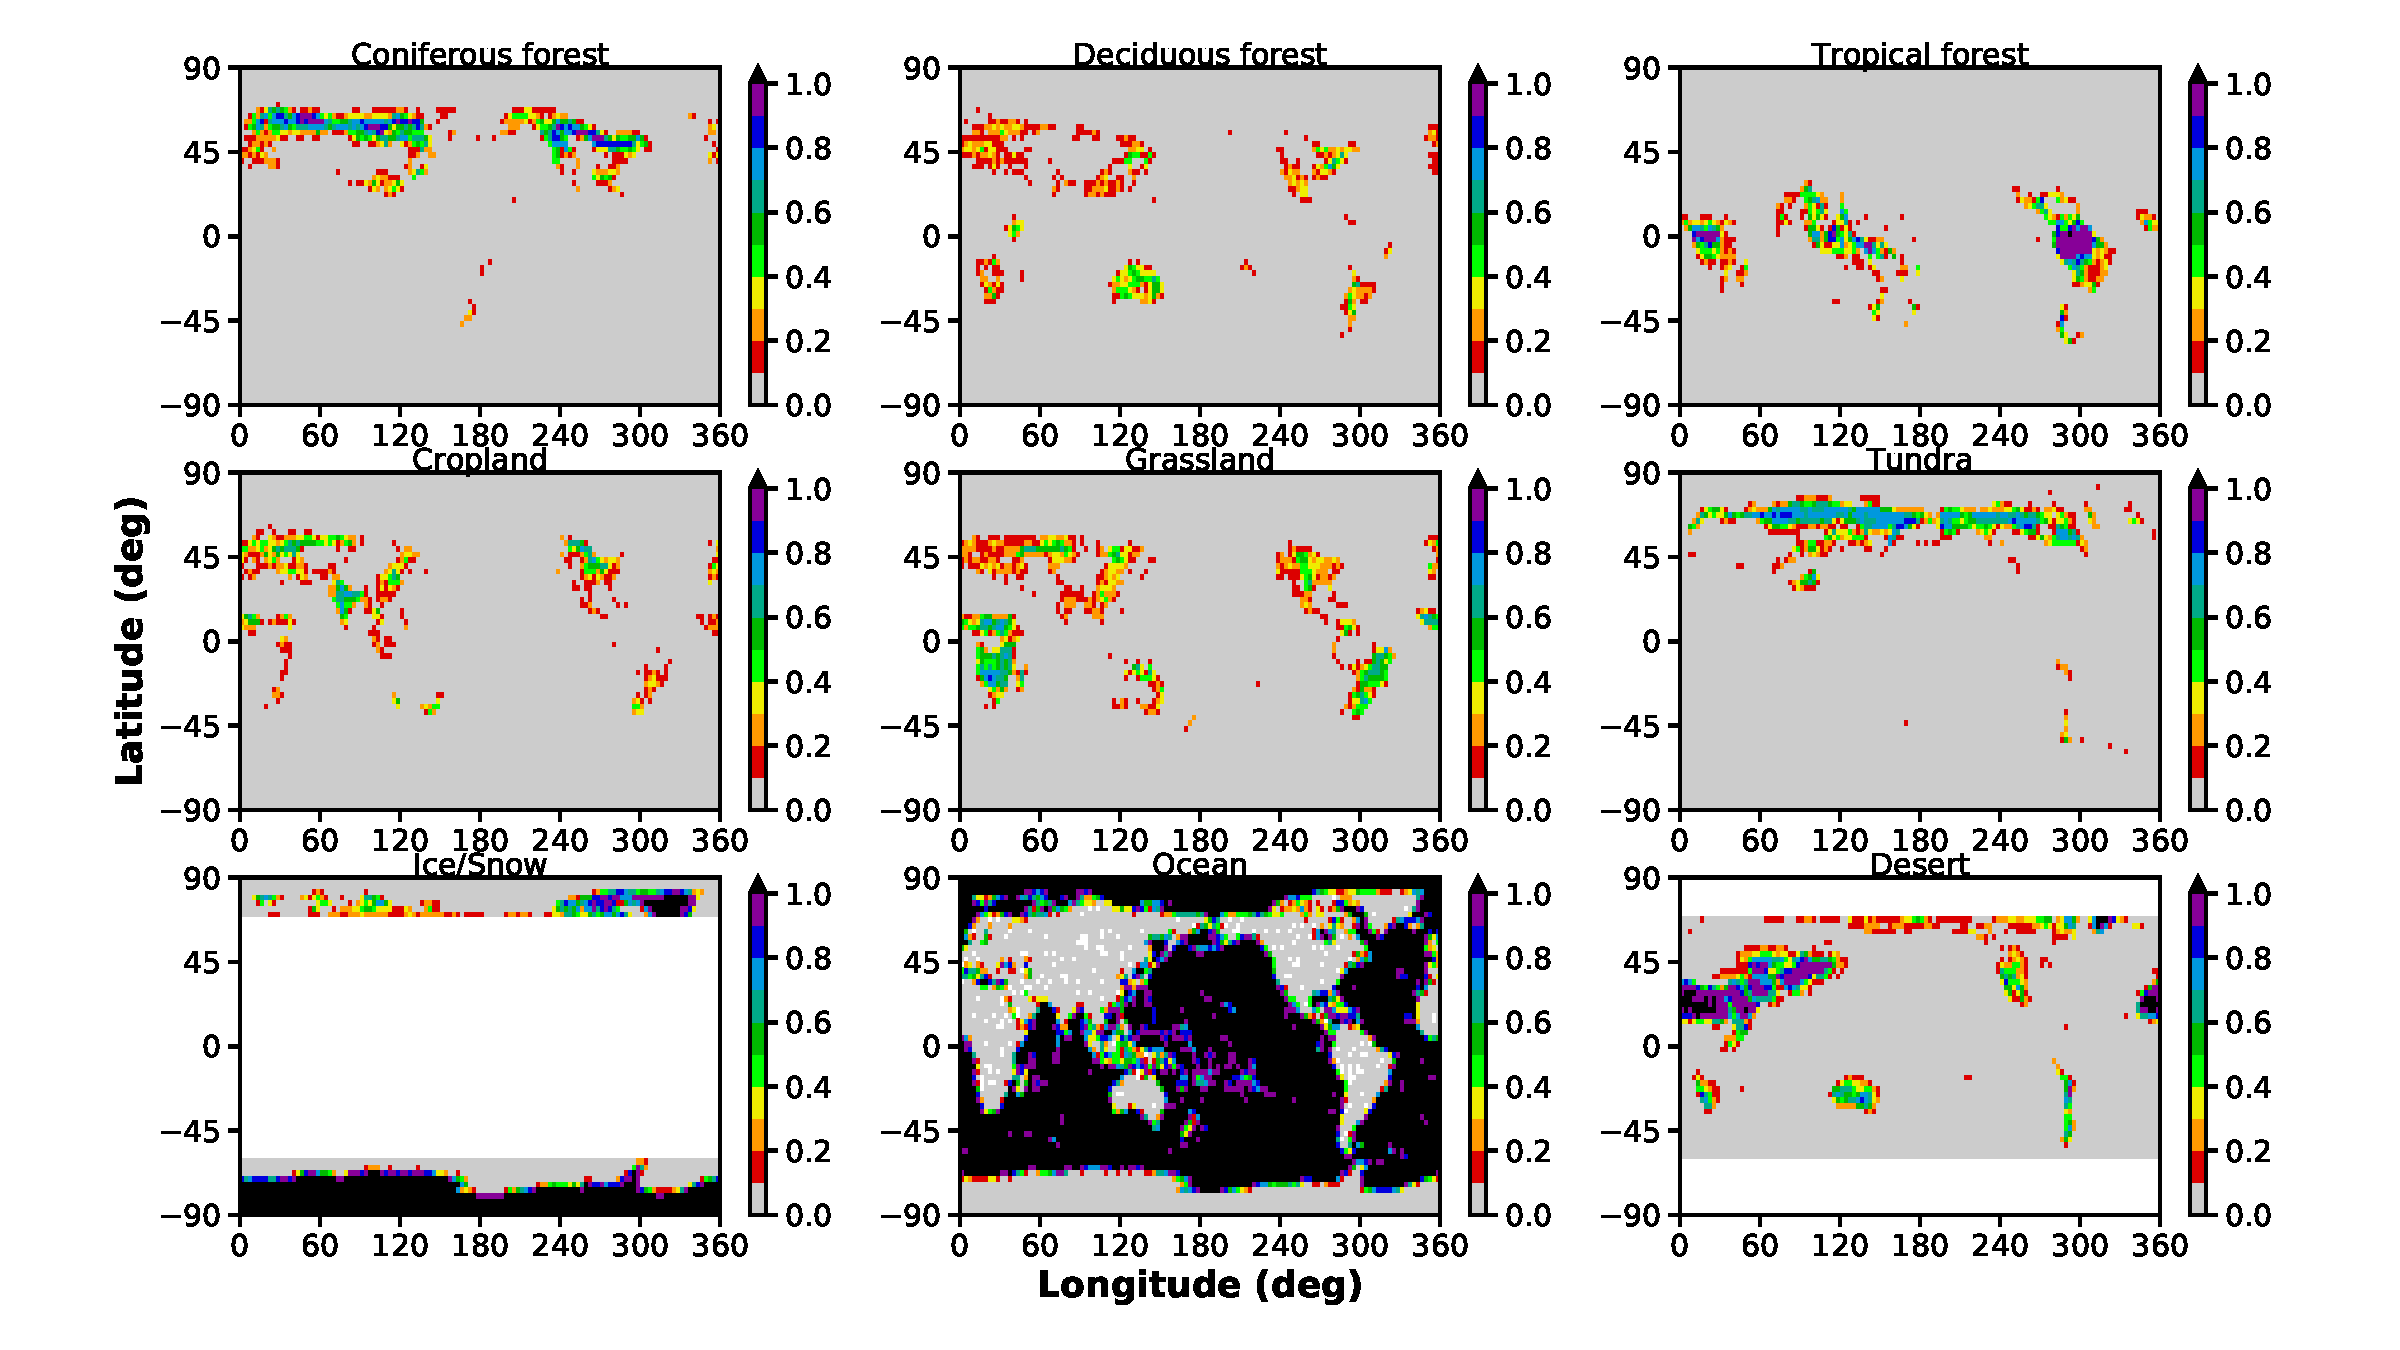
\includegraphics[width=8.3cm]{pictures/pft_categories.pdf}\\
%  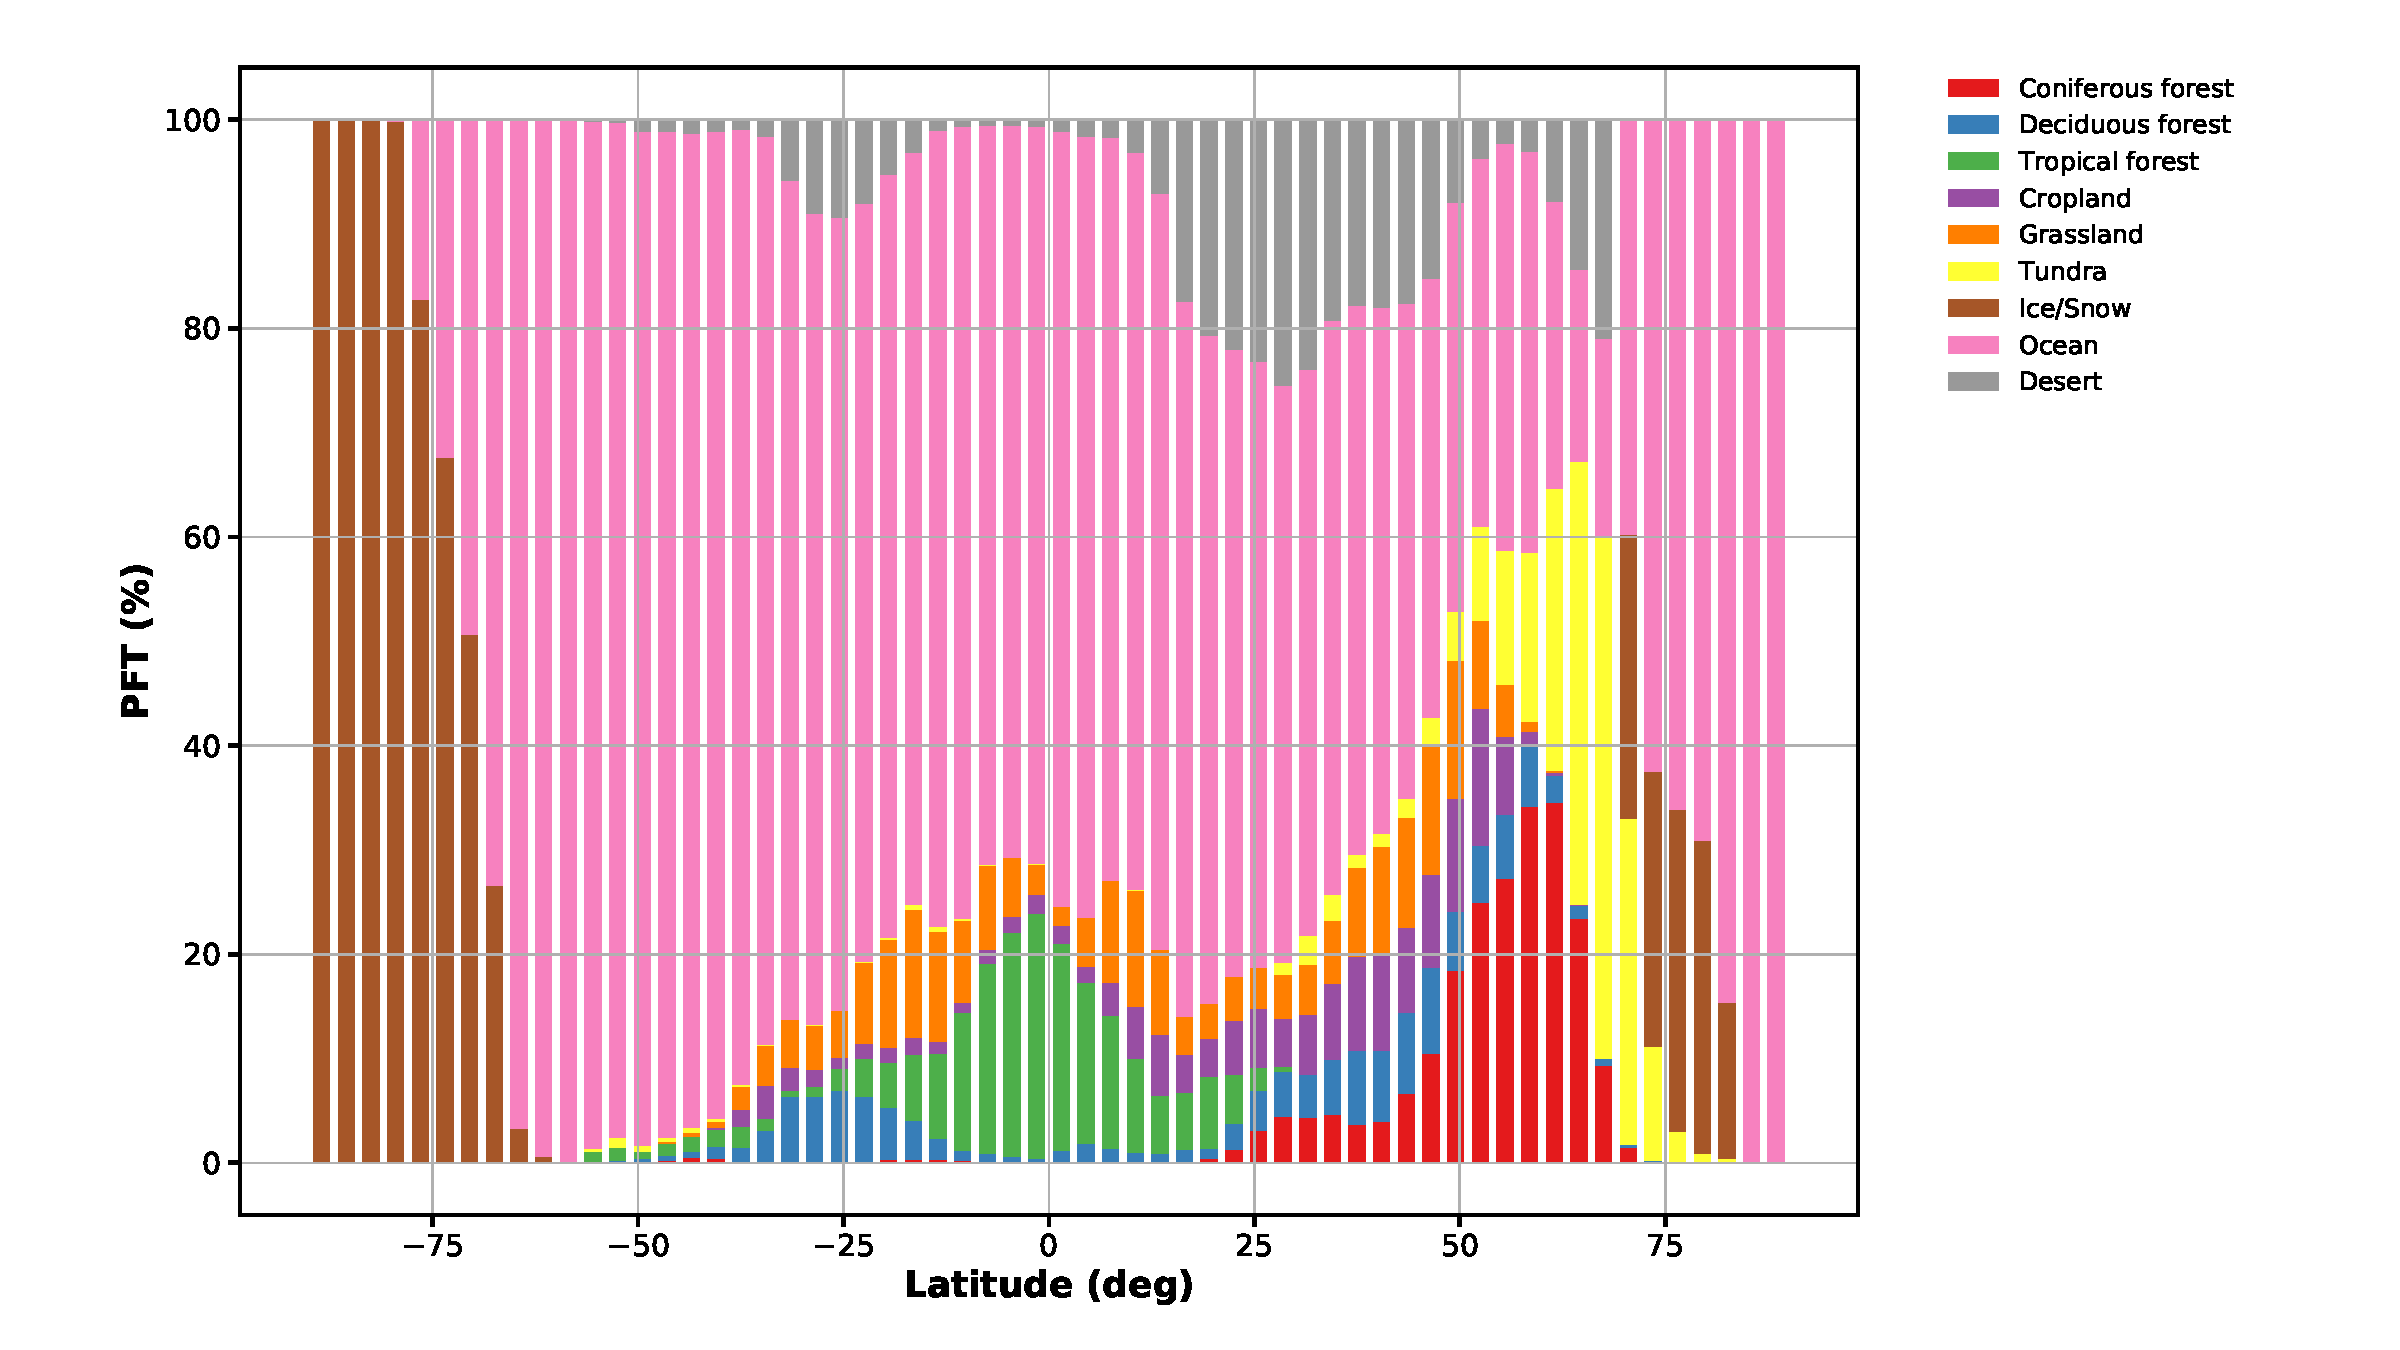
\includegraphics[width=8.3cm]{pictures/pft_categories_zonal.pdf}
%\caption{Plant functional types (PFT). (a) CML2 dynamic landuse 0.5x0.5\,\unit{^\circ}}
%\label{fig:pft_landuse}
%\end{figure}
Mapping of pft landuse types from either ISLSCP2 MODIS or CML2 categories to 9 classical biosphere types used in the EMEP scheme. EMEP categories: Forests, Mediterranean scrub, Crops, Moorland (savanna++), Grassland, Wetlands, Tundra, Desert, Water, Urban
Weighting of conductance with landuse fraction and sum. Inverse of this is gridbox average resistance.

\subsection{Greening season and photosynthetic photon flux density}
\label{subsec:pre-pro}
      {\bf TODO: The neccessary pre-processing routines...}
      
\section{Evaluation}
\label{sec:eval}

\subsection{Sensitivity tests}
\label{subsec:sens}
Include table of all sensitivity runs.
\citep[e.g., $v^\chem{O_3}_{ice/snow} = 1/10000\,\unit{cm s^{-1}}$,][]{ACP:Helmig2007}
dry dep velocity over water \citep{JGR:Helmig2012} Impact of ocean? Although it is a low number there is 2\/3 ocean on earth... (Think, I read this in Hardacre paper... -> Luhar)

\subsection{Comparison with recent multi-model comparison}
\label{subsec:model}
Compare to \citet{ACP:Hardacre2015} as well as \citet{ACP:Luhar2017}.

\subsection{Comparison with observations}
\label{subsec:obs}
The sites used in \citet{ACP:Hardacre2015} and additional ozone zonal data from satellites and sondes (\url{http://bodekerscientific.com/}).

\section{Discussion}
\label{sec:disc}


%\subsection{HEADING}
%\subsubsection{HEADING}



\conclusions  %% \conclusions[modified heading if necessary]
\label{sec:conc}
What did we gain?

%% The following commands are for the statements about the availability of data sets and/or software code corresponding to the manuscript.
%% It is strongly recommended to make use of these sections in case data sets and/or software code have been part of your research the article is based on.

%\codeavailability{TEXT} %% use this section when having only software code available


%\dataavailability{TEXT} %% use this section when having only data sets available


\codedataavailability{TEXT} %% use this section when having data sets and software code available


%\sampleavailability{TEXT} %% use this section when having geoscientific samples available



%\appendix
%\section{}    %% Appendix A

%\subsection{}     %% Appendix A1, A2, etc.


%\noappendix       %% use this to mark the end of the appendix section

%% Regarding figures and tables in appendices, the following two options are possible depending on your general handling of figures and tables in the manuscript environment:

%% Option 1: If you sorted all figures and tables into the sections of the text, please also sort the appendix figures and appendix tables into the respective appendix sections.
%% They will be correctly named automatically.

%% Option 2: If you put all figures after the reference list, please insert appendix tables and figures after the normal tables and figures.
%% To rename them correctly to A1, A2, etc., please add the following commands in front of them:

%\appendixfigures  %% needs to be added in front of appendix figures

%\appendixtables   %% needs to be added in front of appendix tables

%% Please add \clearpage between each table and/or figure. Further guidelines on figures and tables can be found below.



\authorcontribution{Stefanie Falk wrote the paper, did the data analysis, and finalized the implementation of the stomatal conductance in the dry deposition scheme. Amund S{\o}vde Haslerud did most of the implementation and documentation of the updated dry deposition scheme.} %% it is strongly recommended to make use of this section

\competinginterests{The authors declare that they have no conflict of interest.} %% this section is mandatory even if you declare that no competing interests are present

%\disclaimer{TEXT} %% optional section

\begin{acknowledgements}
  This work was supported by the Norwegian Research Council (NRC) through the project The double punch: Ozone and climate stresses on vegetation (OzoNorClim).\\
  We would like to thank Greg Bodeker, Stefanie Kremser (Bodeker Scientific) and Birgit Hassler (DLR) for providing the combined vertical ozone profile database (\url{http://www.bodekerscientific.com}.
  The used Leaf Area Index (LAI) and roughness length ($Z_0$) are available online from Oak Ridge National Laboratory Distributed Active Archive Center, Oak Ridge, Tennessee, U.S.A. (\doi{10.3334/ORNLDAAC/970}).\\
  Community Emission Data System (CEDS) historical emission inventory is provided by the Joint Global Research Institute project (\url{http://www.globalchange.umd.edu/ceds/}.)
\end{acknowledgements}




%% REFERENCES

%% The reference list is compiled as follows:

%% Since the Copernicus LaTeX package includes the BibTeX style file copernicus.bst,
%% authors experienced with BibTeX only have to include the following two lines:
%%
\bibliographystyle{copernicus}
\bibliography{DryDep.bib}
%%
%% URLs and DOIs can be entered in your BibTeX file as:
%%
%% URL = {http://www.xyz.org/~jones/idx_g.htm}
%% DOI = {10.5194/xyz}


%% LITERATURE CITATIONS
%%
%% command                        & example result
%% \citet{jones90}|               & Jones et al. (1990)
%% \citep{jones90}|               & (Jones et al., 1990)
%% \citep{jones90,jones93}|       & (Jones et al., 1990, 1993)
%% \citep[p.~32]{jones90}|        & (Jones et al., 1990, p.~32)
%% \citep[e.g.,][]{jones90}|      & (e.g., Jones et al., 1990)
%% \citep[e.g.,][p.~32]{jones90}| & (e.g., Jones et al., 1990, p.~32)
%% \citeauthor{jones90}|          & Jones et al.
%% \citeyear{jones90}|            & 1990



%% FIGURES

%% When figures and tables are placed at the end of the MS (article in one-column style), please add \clearpage
%% between bibliography and first table and/or figure as well as between each table and/or figure.


%% ONE-COLUMN FIGURES

%%f
%\begin{figure}[t]
%\includegraphics[width=8.3cm]{FILE NAME}
%\caption{TEXT}
%\end{figure}
%
%%% TWO-COLUMN FIGURES
%
%%f
%\begin{figure*}[t]
%\includegraphics[width=12cm]{FILE NAME}
%\caption{TEXT}
%\end{figure*}
%
%
%%% TABLES
%%%
%%% The different columns must be seperated with a & command and should
%%% end with \\ to identify the column brake.
%
%%% ONE-COLUMN TABLE
%
%%t
%\begin{table}[t]
%\caption{TEXT}
%\begin{tabular}{column = lcr}
%\tophline
%
%\middlehline
%
%\bottomhline
%\end{tabular}
%\belowtable{} % Table Footnotes
%\end{table}
%
%%% TWO-COLUMN TABLE
%
%%t
%\begin{table*}[t]
%\caption{TEXT}
%\begin{tabular}{column = lcr}
%\tophline
%
%\middlehline
%
%\bottomhline
%\end{tabular}
%\belowtable{} % Table Footnotes
%\end{table*}
%
%%% LANDSCAPE TABLE
%
%%t
%\begin{sidewaystable*}[t]
%\caption{TEXT}
%\begin{tabular}{column = lcr}
%\tophline
%
%\middlehline
%
%\bottomhline
%\end{tabular}
%\belowtable{} % Table Footnotes
%\end{sidewaystable*}
%
%
%%% MATHEMATICAL EXPRESSIONS
%
%%% All papers typeset by Copernicus Publications follow the math typesetting regulations
%%% given by the IUPAC Green Book (IUPAC: Quantities, Units and Symbols in Physical Chemistry,
%%% 2nd Edn., Blackwell Science, available at: http://old.iupac.org/publications/books/gbook/green_book_2ed.pdf, 1993).
%%%
%%% Physical quantities/variables are typeset in italic font (t for time, T for Temperature)
%%% Indices which are not defined are typeset in italic font (x, y, z, a, b, c)
%%% Items/objects which are defined are typeset in roman font (Car A, Car B)
%%% Descriptions/specifications which are defined by itself are typeset in roman font (abs, rel, ref, tot, net, ice)
%%% Abbreviations from 2 letters are typeset in roman font (RH, LAI)
%%% Vectors are identified in bold italic font using \vec{x}
%%% Matrices are identified in bold roman font
%%% Multiplication signs are typeset using the LaTeX commands \times (for vector products, grids, and exponential notations) or \cdot
%%% The character * should not be applied as mutliplication sign
%
%
%%% EQUATIONS
%
%%% Single-row equation
%
%\begin{equation}
%
%\end{equation}
%
%%% Multiline equation
%
%\begin{align}
%& 3 + 5 = 8\\
%& 3 + 5 = 8\\
%& 3 + 5 = 8
%\end{align}
%
%
%%% MATRICES
%
%\begin{matrix}
%x & y & z\\
%x & y & z\\
%x & y & z\\
%\end{matrix}
%
%
%%% ALGORITHM
%
%\begin{algorithm}
%\caption{...}
%\label{a1}
%\begin{algorithmic}
%...
%\end{algorithmic}
%\end{algorithm}
%
%
%%% CHEMICAL FORMULAS AND REACTIONS
%
%%% For formulas embedded in the text, please use \chem{}
%
%%% The reaction environment creates labels including the letter R, i.e. (R1), (R2), etc.
%
%\begin{reaction}
%%% \rightarrow should be used for normal (one-way) chemical reactions
%%% \rightleftharpoons should be used for equilibria
%%% \leftrightarrow should be used for resonance structures
%\end{reaction}
%
%
%%% PHYSICAL UNITS
%%%
%%% Please use \unit{} and apply the exponential notation


\end{document}
